\newcommand{\E}{\mathbb{E}}
\newcommand{\R}{\mathbb{R}}

\chapter{What Does It Take to Build a Performant Selective Classifier?}
\label{ch:sc_bounds}

% \paperref{\bibentry{rabanser2025what}}

\begin{paperref}
\normalfont
The contents of this chapter consist of research and results taken from: \emph{\bibentry{rabanser2025what}}
\end{paperref}

\section*{Summary}

\looseness=-1
Selective classifiers improve reliability by abstaining on uncertain inputs, yet their performance often lags behind the \emph{perfect-ordering} oracle that accepts examples in exact order of correctness. We formulate this shortfall as a \emph{coverage‑uniform selective‑classification gap} and prove the first finite‑sample decomposition that pinpoints five distinct sources of looseness: Bayes noise, approximation error, ranking error, statistical noise, and implementation or shift‑induced slack. Our bound shows that \emph{monotone} post‑hoc calibration cannot reduce the gap, as it preserves the original score ordering; closing the gap therefore requires scoring mechanisms that can \emph{modify the ranking} induced by the base model. We validate our gap decomposition on synthetic two‐moons data and real‐world vision benchmarks, isolating each error component via controlled experiments. Results confirm that (i) Bayes noise and limited model capacity alone explain large gaps, (ii) only non‑monotone or feature‑aware calibrators shrink the ranking term, and (iii) distribution shift adds a distinct slack that must be addressed by robust training. Together, our decomposition supplies a quantitative \emph{error budget} and concrete design guidelines for building selective classifiers that approach ideal oracle behavior.

\section{Introduction}
\label{sec:intro}

In high-stakes applications like finance~\citep{9260038}, healthcare~\citep{guan2020bounded}, and autonomous driving~\citep{ghodsi2021generating}, machine learning (ML) models are increasingly tasked with making decisions under uncertainty, where dependable predictions are critical. Selective classifiers~\citep{chow1957optimum, el2010foundations} formalize the option to abstain on inputs deemed unreliable, reducing the risk of costly errors by refusing to predict when uncertain. Their effectiveness depends on identifying which predictions to trust and which to defer. A common evaluation metric is the \emph{accuracy–coverage} tradeoff, which quantifies how performance degrades as the model accepts a broader set of inputs. The benchmark is a hypothetical oracle that ranks inputs by their true likelihood of correctness, yielding a \emph{perfect-ordering upper bound}~\citep{geifman2018bias, rabanser2023training}. While some models approach this bound, others fall short—revealing persistent gaps and raising open questions about what properties of the learning setup truly govern selective performance.

\begin{wrapfigure}{R}{0.5\textwidth}
\vspace{-5pt}
    \centering
    \resizebox{\linewidth}{!}{
    \begin{tikzpicture}[
		declare function={}
		]
\begin{axis}[%
  xlabel=Coverage ($c$),
  ylabel=Selective Accuracy,
  xmin = -0.1,
  xmax = 1.1,
  ymin = -0.1,
  ymax = 1.25,
  grid=major,
  width=8cm,
  height=5.5cm,
  tick label style={/pgf/number format/fixed},
  legend style={at={(0.812,1.001)}, anchor=north},]
  
  \newcommand\afull{0.4}
  \newcommand\afullinccoord{{\afull + (1 - \afull)/2}}

  \addplot+[mark={},line width=2pt,Black,name path=C, domain=0:\afull/2] {1};
		  
  \addplot+[mark={},line width=2pt,Black,name path=D, domain=\afull/2:\afull] {15/16*x^2 - 15/8 * x + 107/80};
  
  \addplot+[mark={},line width=2pt,Black,name path=E, domain=\afull:1] {15/16*x^2 - 15/8 * x + 107/80};
  
  \addplot+[mark={},dashed,line width=2pt,Black,name path=A, domain=0:\afull] {1};
  \addplot+[mark={},dashed,line width=2pt,Black,name path=B, domain=\afull:1] {\afull/x};
  \addplot+[draw=none,mark=none,name path=C,domain=0:1] {0};
  \addplot+[Cyan!25!white] fill between[of=A and C,soft clip={domain=0:\afull}];
  \addplot+[Orange!25!white] fill between[of=B and C,soft clip={domain=\afull:1}];
  %\draw [black, line width=1pt, dashed] (\afull,0) -- (\afull, 1.0);
  \node[black, fill=white] at (1,\afull+0.14) {\footnotesize $a_\text{full}$};
  \node[black, fill=white] at (\afull,1.13) {\footnotesize $c = a_\text{full}$};
  

  % \addplot+[black,fill=black] coordinates{(\afull,1)};
  % \addplot+[black,fill=black] coordinates{(1,\afull)};

  \fill[black] (\afull, 1) circle[radius=2.5pt];
  \fill[black] (1,\afull) circle[radius=2.5pt];


  
  
  \addplot+[Black!25!white] fill between[of=A and D,soft clip={domain=0:1}];
  
    \addplot+[Black!25!white] fill between[of=B and E,soft clip={domain=0:1}];
  
  \draw [->, Orange, line width=2pt] (\afull,0.1) -- (1, 0.1);
  \draw [->, Cyan, line width=2pt] (0,0.1) -- (\afull, 0.1);
  \node[Cyan] at (\afull/2,0.25) {\footnotesize correct points};
  \node[Orange] at (\afullinccoord,0.25) {\footnotesize incorrect points};

  \legend{ \scriptsize \realtradeoff,,, \scriptsize \upperbound,,,,, \scriptsize $\int_0^1 \widehat{\Delta}(c)dc$};
 
\end{axis}
\end{tikzpicture}
    }
    \vspace{-12pt}
    \caption[Selective classification gap $\Delta(c)$.]{\textbf{Selective classification gap $\Delta(c)$.}  
      The dashed curve is the oracle frontier \(\overline{\mathrm{acc}}(a_{\text{full}},c)\) under which coverage levels left of \(c=a_{\text{full}}\) (\textcolor{Cyan}{blue}) accept correct predictions first, and rank incorrect predictions last (\textcolor{Orange}{orange}). The solid curve shows the realized selective accuracy \(\mathrm{acc}_{c}(h,g)\).  
      The mismtach between \(\overline{\mathrm{acc}}(a_{\text{full}},c)\) and \(\mathrm{acc}_{c}(h,g)\) at coverage $c$ is the gap \(\Delta(c)\);  
      the gray area visualizes the gap area over the full coverage spectrum.}
      \vspace{-25pt}
    \label{fig:bounds_overview}
\end{wrapfigure}

Classical theory explains selective classification in two idealized regimes. In the \emph{realizable} setting~\citep{el2010foundations}, where the data is noiseless and the true predictor lies within the hypothesis class, the model can asymptotically achieve the perfect accuracy–coverage curve. In the more general \emph{agnostic} setting~\citep{wiener2011agnostic}, the classifier competes with the best-in-class predictor, but this benchmark may itself fall well below the oracle bound—and the theory does not isolate the source of the gap. As a result, even the strongest formal guarantees offer little practical guidance:
\begin{quote}
\centering
\emph{For my finite model on finite data, what aspects of the learning setup will actually move my trade-off curve closer to the upper bound?}
\end{quote}

To answer this question, we re‑frame selective performance around the \emph{selective classification
gap}~\(\Delta(c)\): the mismatch between a model’s accuracy–coverage curve and the oracle
bound (see Figure~\ref{fig:bounds_overview} for an illustrative example). 
We show that this gap admits a finite‑sample decomposition:
\begin{equation}
\label{eq:intro-gap}
\widehat{\Delta}(c)
\;\le\;
\underbrace{\varepsilon_{\text{Bayes}}(c)}_{\text{\scriptsize irreducible}}
+\;\underbrace{\varepsilon_{\text{approx}}(c)}_{\text{\scriptsize capacity}}
+\;\underbrace{\varepsilon_{\text{rank}}(c)}_{\text{\scriptsize ranking}}
+\;\underbrace{\varepsilon_{\text{stat}}(c)}_{\text{\scriptsize data}}
+\;\underbrace{\varepsilon_{\text{misc}}(c)}_{\text{\scriptsize optimization\;\&\;shift}},
\qquad\forall c\in(0,1].
\end{equation}

Each term corresponds to a distinct—and often \emph{measurable}—source of looseness. 
The first term, \(\varepsilon_{\text{Bayes}}(c)\), reflects irreducible uncertainty: if the true label is inherently unpredictable from the input (e.g., due to label noise), even a perfect classifier must abstain on some examples. 
Next, \(\varepsilon_{\text{approx}}(c)\) captures limits of the model class: if the function class is too weak to approximate the Bayes-optimal decision rule, the gap widens. 
The third term, \(\varepsilon_{\text{rank}}(c)\), quantifies the model’s failure to correctly order inputs by their likelihood of correctness—typically due to poor confidence estimation or miscalibration. 
The statistical term \(\varepsilon_{\text{stat}}(c)\) accounts for finite-sample fluctuations that affect both learning and evaluation. 
Finally, \(\varepsilon_{\text{misc}}(c)\) aggregates practical imperfections, such as optimization error or test-time distribution shift. Equation~\eqref{eq:intro-gap} thus provides a coverage-uniform ``error budget'' that transforms the qualitative question posed earlier into a concrete quantitative diagnosis.

\looseness=-1
Two insights, developed further in later sections, are worth previewing. First, monotone post‑hoc calibration cannot reduce the \emph{ranking} term \(\varepsilon_{\text{rank}}(c)\), as it preserves the total order of scores—leaving the accuracy–coverage curve unchanged. Second, Equation~\eqref{eq:intro-gap} serves as an \emph{error budget} that identifies cost‑effective levers: (i) increase capacity or distill from a more expressive teacher to shrink \(\varepsilon_{\text{approx}}\); (ii) use additional or repeated labels and noise‑robust losses to reduce \(\varepsilon_{\text{Bayes}}\); (iii) enlarge validation data to lower \(\varepsilon_{\text{stat}}\); and (iv) apply domain adaptation or importance weighting to address \(\varepsilon_{\text{misc}}\).

\textbf{Contributions.}
We summarize our main contributions below:
% \vspace{-5pt}
\begin{itemize}
    \item \textbf{Problem formulation.}  
          We recast selective prediction in terms of a \emph{coverage‑uniform selective‑classification gap}—the key quantity to minimize to approach oracle behavior.  
This framing unifies prior work and highlights which failure modes dominate at each coverage level.

    \item \textbf{Theoretical analysis.}  
          We present the first \emph{finite‑sample decomposition} of the gap (Eq.~\eqref{eq:intro-gap}), dividing it into five terms: Bayes, approximation, ranking, statistical, and miscellaneous errors.  
Our analysis further shows that \emph{monotone calibration cannot reduce the gap}, motivating ranking‑aware methods.

\item \textbf{Empirical validation.}  
      Experiments—from two‑moons to large‑scale vision—confirm the decomposition: Bayes noise and capacity limits drive large gaps; temperature scaling improves calibration but not ranking; and shift-aware methods remain essential under distribution shift. \emph{These results clarify which factors matter most and how to target them effectively in practice.}
\end{itemize}

\section{Background \& Related Work}
\label{sec:background}

Selective classification extends the standard supervised classification framework as follows:

\begin{definition}[Selective Classifier~\citep{chow1957optimum, el2010foundations}]
A selective classifier is a pair \( (h, g) \), where \( h: \mathcal{X} \to \mathcal{Y} \) is a classifier over covariates \( \mathcal{X} = \mathbb{R}^D \) and labels \( \mathcal{Y} = \{1, \ldots, K\} \), and \( g: \mathcal{X} \times (\mathcal{X} \to \mathcal{Y}) \to \mathbb{R} \) is a selection function that assigns a confidence score.  
Given a threshold \( \tau \in \mathbb{R} \), the model abstains when the score falls below the threshold:
\begin{equation}
    \label{eq:sel_class}
    (h, g)(x) = \begin{cases}
    h(x) & \text{if } g(x, h) \geq \tau \\
    \bot & \text{otherwise}
    \end{cases}
    \enspace .
\end{equation}
\end{definition}

Intuitively, a selective classifier predicts only when confident.  
The selection score \(g(x, h)\) determines whether to accept or abstain: if \(g(x, h) \geq \tau\), the model outputs \(h(x)\); otherwise, it returns \(\bot\).

Many prior works have developed selective classification methods for training competitive pairs \((h, g)\).  
A popular selective prediction method is \emph{Softmax Response} (\sr)~\citep{hendrycks2016baseline, geifman2017selective}, which uses classifier confidence as the selection score.  
To improve calibration and reduce predictive variance, ensembling approaches have been explored: \emph{Deep Ensembles} (\de)~\citep{lakshminarayanan2017simple} train multiple models with different initializations, while \emph{Selective Classification via Training Dynamics} (\sctd)~\citep{rabanser2022selective} ensembles intermediate checkpoints.  
Other methods—such as \emph{SelectiveNet} (\sn)\citep{geifman2019selectivenet}, \emph{Deep Gamblers} (\dg)\citep{liu2019deep}, and \emph{Self-Adaptive Training} (\sat)~\citep{huang2020self}—alter the model architecture or loss function ensuring that prediction and rejection are learned jointly.




The efficacy of a selective classifier is evaluated using the empirical accuracy-coverage tradeoff.

\begin{definition}[Empirical Accuracy–Coverage Tradeoff]
\label{def:emp_acc_cov}
Let \(D=\{(x_i,y_i)\}_{i=1}^N\) be a dataset.  For a selective classifier \((h,g)\) and threshold \(\tau\), define
\begin{align}
\label{eq:emp_coverage}
\hat{\xi}_{h,g}(\tau)
&= \frac{1}{N}\,\bigl|\{\,i : g(x_i,h) \ge \tau \}\bigr|,
\\[6pt]
\label{eq:emp_accuracy}
\hat{\alpha}_{h,g}(\tau)
&= 
\begin{cases}
\displaystyle
\frac{\bigl|\{\,i : h(x_i)=y_i \text{ and } g(x_i,h) \ge \tau \}\bigr|}{
      \bigl|\{\,i : g(x_i,h) \ge \tau \}\bigr|}, 
& \text{if } \hat{\xi}_{h,g}(\tau)>0,\\[10pt]
0, & \text{if } \hat{\xi}_{h,g}(\tau)=0.
\end{cases}
\end{align}
The pair \((\hat{\xi}, \hat{\alpha})\) as \(\tau\) varies is the empirical accuracy–coverage curve.
\end{definition}
% \mnote{Should the def be titled 'curve' rather than 'tradeoff'? Usually tradeoff refers to a concrete result about the curve}
The score \(g(x,h)\) therefore induces a total order over \(D\): \(x_1\) is accepted before \(x_2\) if \(g(x_1,h) > g(x_2,h)\).  
This ordering governs which inputs are retained as coverage decreases.  
Effective strategies aim to maximize \(\hat{\alpha}\) at each coverage level \(\hat{\xi}\), often trading off accuracy and coverage.

%\my{I think you need to specify that you are not assuming a batched setting at all here. A total order is only meaningful if at every point, you can see all the samples at once.}
% \my{Also maybe motivate why we care about the induced ordering here? make the transition smoother that is.}


\paragraph{Accuracy–coverage tradeoff evaluation.}
The accuracy–coverage tradeoff is often summarized by the area under the accuracy–coverage curve (\texttt{AUACC}), integrating selective accuracy over all coverage levels. However, \citet{geifman2018bias} show that \texttt{AUACC} favors models already accurate at full coverage. To address this issue, \citet{geifman2018bias} and \citet{rabanser2023training} propose oracle-based bounds, which become loose at low utility~\citep{galil2023can}. To avoid accuracy bias, \citet{galil2023can} and \citet{pugnana2023auc} recommend using the classifier’s \texttt{AUROC} instead. But \texttt{AUROC} is not monotonic in \texttt{AUACC}~\citep{cattelan2023fix, ding2020revisiting}, thus favoring methods tuned for \texttt{AUROC} over selective accuracy. Earlier work~\citep{el2010foundations, wiener2011agnostic} characterizes optimal selective classifiers in both realizable and agnostic regimes but focuses on existence rather than practical instantiation—unlike our finite-sample perspective.



\section{Decomposing the Selective Classification Gap To Optimality}
\label{sec:methods}

We characterize the optimal performance achievable by a selective classifier given its full-coverage accuracy, establishing a reference against which all practical selective classifiers can be evaluated.


\subsection{Oracle Bound and Selective Classification Gap}

\begin{definition}[Perfect Ordering Upper Bound~\citep{geifman2018bias, rabanser2023training}]
\label{def:poub}
Fix a base classifier \(h\) whose full‑coverage (standard) accuracy is
\(a_{\text{full}}:=\Pr\bigl(h(X)=Y\bigr)\in[0,1]\).
For any desired coverage level \(c\in(0,1]\), the best selective
accuracy—achieved by accepting the \(c\)-fraction of points with the \emph{highest}
posterior correctness $\Pr(h(X)=Y\mid X)$—is
\begin{equation}
\label{eq:bound}
\overline{\mathrm{acc}}\bigl(a_{\text{full}},c\bigr)
=\;
\begin{cases}
1, & 0 < c \le a_{\text{full}}, \\[6pt]
\dfrac{a_{\text{full}}}{c}, & a_{\text{full}} < c < 1.
\end{cases}
\end{equation}
\end{definition}

This piecewise curve (see Figure~\ref{fig:bounds_overview}) traces an \emph{oracle} accuracy–coverage frontier, assuming access to a perfect ranking of examples by correctness probability. Any real selective classifier falls below this bound—potentially far below, depending on its calibration, expressivity, and sensitivity to noise. To quantify how far a given classifier falls short of this ideal, we define the \emph{selective classification gap}.

\begin{definition}[Selective Classification Gap]
\label{def:gap}
Let \((h,g)\) be a selective classifier with full‑coverage accuracy 
\(a_{\mathrm{full}}=\Pr(h(X)=Y)\).  For a coverage level \(c\in(0,1]\), let
\(\tau_c\) be the threshold satisfying \(\Pr\bigl(g(X,h)\ge\tau_c\bigr)=c\).  The selective accuracy at coverage \(c\) is
\(
\mathrm{acc}_c(h,g)
:=
\Pr\bigl(h(X)=Y \;\bigm|\; g(X,h)\ge\tau_c\bigr).
\)
The selective classification gap at coverage \(c\) is then defined as the deviation from the perfect-ordering upper bound:
\begin{equation}
\Delta(c)
:=
\overline{\mathrm{acc}}\bigl(a_{\mathrm{full}},c\bigr)
\;-\;\mathrm{acc}_c(h,g).
\end{equation}
\end{definition}

The function \(\Delta(c)\) offers a coverage-resolved diagnostic of selective performance. A small gap indicates near-oracle behavior—accepting only examples it can confidently and correctly classify—while a large gap suggests limitations in estimating correctness or ranking examples reliably. Understanding the magnitude and shape of this gap is key to analyzing and improving selective classifiers.

\subsection{Why Is the Upper Bound Loose?}
\label{sec:why-loose}

The oracle bound in Definition~\ref{def:poub} relies on two idealized
assumptions: perfect prediction on all inputs and perfect ranking by
the true correctness posterior. In practice, selective classifiers deviate in
four principal ways, each corresponding to a term in our later
decomposition (\(\varepsilon_{\text{Bayes}},\varepsilon_{\text{approx}},
\varepsilon_{\text{rank}},\varepsilon_{\text{stat}}\)):

\begin{enumerate}

\item \textbf{Bayes noise (\(\varepsilon_{\text{Bayes}}\)).}  
  Even a Bayes-optimal rule errs on intrinsically ambiguous points
(where \(\max_y \Pr(Y=y\mid X)<1\)), unavoidable in real data~\citep{devroye2013probabilistic}.  
As coverage increases, the oracle must accept some of these noisy inputs, lowering the achievable accuracy.


\item \textbf{Approximation limits (\(\varepsilon_{\text{approx}}\)).}  
  A learned model \(h\) drawn from a restricted hypothesis class may
  misclassify inputs with high posterior confidence under the Bayes rule~\citep{bishop2006pattern}.  
  This gap reduces full-coverage accuracy and limits selective performance.

\item \textbf{Ranking error (\(\varepsilon_{\text{rank}}\)).}  
  Let \(\eta_h(x):=\Pr\bigl(h(x)=Y\mid X=x\bigr)\) denote the true
  correctness posterior. The confidence score \(g(X,h)\) may
  mis-order inputs relative to \(\eta_h(x)\), leading easy examples
  to be rejected and harder ones accepted, which increases \(\Delta(c)\).  

\item \textbf{Statistical noise (\(\varepsilon_{\text{stat}}\)).}  
  Estimating the threshold \(\tau_c\) and selective accuracy from a finite validation set introduces randomness
  of order \(\mathcal{O}(\sqrt{\log(1/\delta)/n})\). This follows from concentration bounds; see~\citet{shalev2014understanding} for standard applications in learning theory.

\end{enumerate}

\begin{takeaway}
The selective classification gap \(\Delta(c)\) reflects a mix of irreducible noise,
model misspecification, ranking errors, and sampling variability. Addressing each—via cleaner labels,
stronger models, or improved ranking—can tighten selective prediction performance.
\end{takeaway}

\looseness=-1
Next, we formalize this decomposition and provide a general bound on the total gap.

\subsection{Formal Decomposition of the Gap}
\label{sec:formal-gap}

We now give a principled decomposition of the selective classification gap and provide a corresponding finite-sample upper bound. For clarity and notational simplicity, we treat the binary‑label case \(\mathcal{Y}=\{0,1\}\); the multiclass extension follows by a standard one‑vs‑rest reduction.

\textbf{Notation.} Let \(\eta(x):=\Pr\bigl(Y=1\mid X=x\bigr)\) be the Bayes posterior.
For a fixed classifier \(h:\mathcal{X}\to\mathcal{Y}\) define its
(induced) correctness posterior
\begin{equation}
  \eta_h(x)\;:=\;\Pr\bigl(h(x)=Y\mid X=x\bigr)
  \;=\;\eta(x)\,\mathbb{I}_{\{h(x)=1\}}+
        \bigl(1-\eta(x)\bigr)\mathbb{I}_{\{h(x)=0\}}.
\end{equation}
All expectations and probabilities are taken w.r.t.\ the true data distribution
\(\mathcal{D}\). Throughout let \(g(x,h)\) be the confidence score.
For a target coverage \(c\in(0,1]\) denote by
\begin{equation}
  t_c \quad \text{s.t.}\quad
  \Pr\bigl(g(X,h)\ge t_c\bigr)=c
\end{equation}
the \emph{population threshold}, and write the
\emph{accepted region}
\(A_c:=\{x:g(x,h)\ge t_c\}\).  
The oracle that attains the perfect‑ordering bound accepts $A_c^{\star}:=\bigl\{x:\eta_h(x)\text{ is among the largest }c\text{-fraction}\bigr\}$.

\textbf{Error Terms.} We isolate the following sources of error affecting selective prediction performance:
\begin{align}
\varepsilon_{\text{Bayes}}(c)
&:=\E\Bigl[1-\max\{\eta(X),1-\eta(X)\}\;\Bigm|\;X\in A_c\Bigr],
\\[4pt]
\varepsilon_{\text{approx}}(c)
&:=\E\Bigl[\bigl|\eta_h(X)-\eta(X)\bigr|\;\Bigm|\;X\in A_c\Bigr],
\\[4pt]
\varepsilon_{\text{rank}}(c)
&:=\E\bigl[\eta_h(X)\mid X\in A_c^{\star}\bigr]
  -\E\bigl[\eta_h(X)\mid X\in A_c\bigr]\;\;\;\;\;\;(\ge0),
\\[4pt]
\varepsilon_{\text{stat}}(c)
&:=C\sqrt{\frac{\log(1/\delta)}{n}},
\end{align}
where \(n\) is the evaluation‑set size, \(\delta\in(0,1)\) a confidence
parameter, and \(C>0\) an absolute constant. Intuitively, \(\varepsilon_{\text{Bayes}}\) is the irreducible label noise inside the accepted region; \(\varepsilon_{\text{approx}}\) measures how far \(h\) is from Bayes‑optimal on the \emph{selected} inputs; and \(\varepsilon_{\text{rank}}\) is a \emph{ranking regret}—the accuracy loss due solely to picking the wrong \(c\)-fraction of examples.

\begin{remark}[Distance to a Perfect Ranker]
A natural way to gauge how far the learned acceptance rule is from the oracle is
the mass mis-ordered
\begin{equation}
    D_{\text{rank}}(c)\;:=\;
    \Pr\bigl(X\in A_c^{\star}\setminus A_c\bigr)
    +\Pr\bigl(X\in A_c\setminus A_c^{\star}\bigr).
\end{equation}
It equals the total probability of examples that would have to be
\emph{swapped} between $A_c$ and $A_c^{\star}$ to recover perfect ordering.
Hence $D_{\text{rank}}(c)=0$ iff $A_c=A_c^{\star}$, in which case
$\varepsilon_{\text{rank}}(c)$ also vanishes.
\end{remark}

\begin{theorem}[Selective Gap Bound]
\label{thm:gap}
For a coverage level \(c\in(0,1]\) and a selective classifier \((h,g)\) the population gap obeys
\begin{equation}
\Delta(c)=\overline{\mathrm{acc}}\bigl(a_{\mathrm{full}},c\bigr)
-\mathrm{acc}_c(h,g)
\;\le\;
\varepsilon_{\text{Bayes}}(c)
+\varepsilon_{\text{approx}}(c)
+\varepsilon_{\text{rank}}(c).
\label{eq:pop-gap-ranking}
\end{equation}
Let \(\widehat{\Delta}(c)\) be the empirical gap on \(n\) i.i.d.\
test points.  Then, with probability at least \(1-\delta\),
\begin{equation}
\widehat{\Delta}(c)
\;\le\;
\varepsilon_{\text{Bayes}}(c)
+\varepsilon_{\text{approx}}(c)
+\varepsilon_{\text{rank}}(c)
+C\sqrt{\tfrac{\log(1/\delta)}{n}}.
\label{eq:emp-gap-ranking}
\end{equation}
% where \(C>0\) is an absolute constant.
\end{theorem}

\begin{proof}
Because
\(
\mathrm{acc}_c(h,g)=\E[\eta_h(X)\mid A_c],
\)
the gap decomposes as
\[
  \Delta(c)
  =\underbrace{\E[\eta_h\mid A_c^{\star}]
               -\E[\eta_h\mid A_c]}_{\varepsilon_{\text{rank}}(c)}
   \;+\;
   \underbrace{\E[\eta_h-\mathbb{I}_{\{h=Y\}}\mid A_c]}
              _{\varepsilon_{\text{approx}}(c)}
   \;+\;
   \underbrace{\E[1-\max\{\eta,1-\eta\}\mid A_c]}
              _{\varepsilon_{\text{Bayes}}(c)}.
\]
This yields the population bound \eqref{eq:pop-gap-ranking}. 
For each expectation in the decomposition apply Hoeffding’s
inequality, a union bound over the three terms gives, with probability
\(1-\delta\),
\(
  |\widehat{\Delta}(c)-\Delta(c)|
  \le C\sqrt{\log(1/\delta)/n}.
\)
Adding this deviation to \eqref{eq:pop-gap-ranking} establishes
\eqref{eq:emp-gap-ranking}. \\See Appendix~\ref{app:proof-gap-ranking} for an extended proof with detailed intermediate steps.
\end{proof}

\subsection{Calibration and Its (Limited) Effect on the Gap}
\label{sec:calibration-gap}

As shown in Theorem~\ref{thm:gap}, the selective classification gap includes a \emph{ranking error} term \(\varepsilon_{\text{rank}}(c)\), which captures misalignment between the confidence score and true correctness. Model calibration~\citep{niculescu2005predicting}—widely used to reduce over- or underconfidence—is often assumed to improve this alignment by transforming scores to better reflect correctness likelihood. Yet its effect on selective performance remains ambiguous and context-dependent. Prior work has reached conflicting conclusions: \citet{zhu2022rethinking} argue that calibration may degrade abstention behavior, while \citet{galil2023can} find that temperature scaling can improve selective prediction in practice. We show that the impact on the gap depends critically on the \emph{type} of calibration method used and its influence on the induced ranking. We begin by recalling the formal definition of calibration.

\begin{definition}[Perfect Calibration]
\label{def:calibration}
For each input \(x\) let a model produce a predicted label \(\hat y(x)\) and an associated confidence score \(s(x)\in[0,1]\). We say the model is perfectly calibrated if
\begin{equation}
  \Pr\bigl(Y = \hat y(X)\;\bigm|\;s(X)=t\bigr) \;=\; t \qquad \text{for every confidence level}\ t\in[0,1].
  \label{eq:perfect-cal}
\end{equation}
\end{definition}

Practical estimators approximate~\eqref{eq:perfect-cal} via a post-hoc map \(\phi\) such that \(\tilde s(x)=\phi(s(x))\) approaches prefect calibration. \emph{Expected Calibration Error (ECE)}~\citep{naeini2015obtaining} quantifies this closeness:
\begin{equation}
  \text{ECE} = \sum_{b=1}^B \frac{|I_b|}{n}
  \left| \frac{1}{|I_b|} \sum_{i \in I_b} \mathbb{I}\{ \hat y(x_i) = y_i \}
         - \frac{1}{|I_b|} \sum_{i \in I_b} \tilde s(x_i) \right|,
  \label{eq:ece}
\end{equation}
where \(I_b\) is the set of indices in bin \(b\), \(n\) is the total number
of examples, and \(B\) is the number of bins.

\textbf{Monotone Score-Level Calibration Leaves the Gap Intact.}
Temperature scaling~\citep{guo2017calibration}, isotonic regression~\citep{zadrozny2002transforming}, and histogram
binning~\citep{zadrozny2001obtaining} all fit a \emph{monotone} \(\phi\colon[0,1]\to[0,1]\) that preserves score ordering.
Because monotone maps preserve ordering,
the acceptance set
\(A_c=\{x:\tilde s(x)\ge\tau_c\}\)
is identical to the one obtained from \(s(x)\);
hence the selective accuracy
\(\mathrm{acc}_c(h,g)\)
and the gap
\(
\Delta(c)=\overline{\mathrm{acc}}\bigl(a_{\text{full}},c\bigr)-\mathrm{acc}_c(h,g)
\)
are \emph{unchanged}.
Monotone calibration thereby reduces the approximation error \(\varepsilon_{\text{approx}}(c)\) in Section~\ref{sec:formal-gap} but leaves the ranking error \(\varepsilon_{\text{rank}}(c)\) untouched.

\textbf{Why Temperature Scaling \texorpdfstring{\emph{Can}}{} Reorder But Rarely Does.}
Temperature scaling, the most widely used post-hoc calibration technique, divides every logit vector
\(z(x)\in\mathbb{R}^K\) by a scalar \(T>0\),
\begin{equation}
p_j^{(T)}(x)=
\frac{\exp(z_j(x)/T)}{\sum_k \exp(z_k(x)/T)}.
\end{equation}
Two inputs with different logit \emph{margins} can swap their
max-probability after rescaling. In theory this breaks the monotone
ranking guarantee; in practice such ties occur only when the runner-up logit gaps are extremely small. Consequently, the induced change in the
accuracy–coverage curve is negligible—a pattern we also observe empirically. See Appendix~\ref{app:ts-rerank} for an extended discussion.

\textbf{Moving the Gap Requires Non-Monotone Scoring.}
To reduce the selective classification gap \(\Delta(c)\), one must go beyond simple monotone calibration and actively modify the acceptance ordering through one of the following approaches:

% \vspace{-5pt}
\begin{itemize}
    \item \textbf{Adaptive, ensemble, or feature-aware scoring}:  
          Techniques such as self-adaptive training (\(\texttt{SAT}\)), deep ensembles (\(\texttt{DE}\)), and learned calibration heads \(g_\psi(x)\) predict correctness scores from hidden representations or multiple model votes. These approaches leverage instance-specific uncertainty and shared feature context to rerank samples that otherwise receive similar raw confidence values.
          
\item \textbf{Binning or resampling}:  
      Techniques such as Bayesian Binning into Quantiles (BBQ)~\citep{naeini2015obtaining} and conformal p-value methods~\citep{angelopoulos2021gentle} refine confidence scores by estimating accuracy over adaptive data subsets. Both use empirical statistics—either at the bin level or per example—to recalibrate and reorder predictions, often improving ranking.


\item \textbf{Vector/Dirichlet scaling}:  
      A non-monotone transformation of the logit vector \(z\) via a learned affine map \(Wz + b\), with \(W \in \mathbb{R}^{K \times K}\), enables reordering of confidence scores by capturing inter-class dependencies, nonlinear score interactions, and representation-sensitive shifts~\citep{kull2019beyond}.



\end{itemize}

\looseness=-1
\textbf{Loss Prediction as a Multicalibration Litmus Test.}
A complementary view on how calibration connects to ranking ability starts from \emph{multicalibration}~\citep{hebert2018multicalibration},
the degree to which a model is calibrated on select subgroups. Recent work by \citet{gollakota2025loss} shows that strong multicalibration is closely tied to a model's ability to \emph{predict its own loss}, an idea seemingly closely related to selective prediction. We formalize this connection in Appendix~\ref{app:loss-pred} and show, both theoretically and empirically, that success or failure at the loss-prediction task corresponds directly to the magnitude of the ranking error \(\varepsilon_{\text{rank}}(c)\). In short, if a model's confidence scores cannot be out-predicted on their own mistakes, they are effectively multicalibrated—and near the oracle frontier.

\begin{takeaway}
Monotone score-level calibration (e.g., temperature scaling) is not enough to reduce the selective classification gap. Closing the gap requires scoring methods that actively change the ranking—through feature-aware heads, ensembles, or non-monotone transformations.
\end{takeaway}


\subsection{Additional Practical Sources of Looseness}
\label{sec:extra-slack-short}
The decomposition in Theorem~\ref{thm:gap} captures the \emph{intrinsic} sources of error—Bayes noise, approximation limits, ranking error, and sampling slack—forming a principled bound that holds even under perfect optimization, infinite data, and i.i.d.\ testing. In practical deployments, however, additional imperfections can inflate the empirical gap \(\widehat{\Delta}(c)\). These stem from implementation details, scoring granularity, and distribution shift—not fundamental limits, but contingent slack terms reducible through better engineering. We summarize them below under a single \emph{residual slack} term \(\varepsilon_{\text{misc}}(c)\).
\begin{enumerate}
  \item \textbf{Optimization error \(\varepsilon_{\text{opt}}\).}  
    In practice, gradient‐based solvers rarely attain the empirical risk minimizer. If \(L(\theta)\) denotes the end-to-end training objective—encompassing model architecture, loss (e.g.\ cross-entropy), and training data—and \(\hat\theta\) its final iterate, then $\varepsilon_{\text{opt}}\;=\; L(\hat\theta) \;-\; \min_{\theta}L(\theta)$, which—via standard surrogate‐to‐0/1 calibration bounds—translates into a nonzero selective‐accuracy loss that persists even under infinite data.
  \item \textbf{Distribution shift \(\varepsilon_{\text{shift}}(c)\).}  
  When the test distribution \(p_{\mathrm{test}}\) deviates from the training distribution \(p_{\mathrm{train}}\), both calibration and ranking typically degrade. In particular, for a hypothesis class \(\mathcal{H}\), the gap due to shift can be bounded by an \emph{Integral Probability Metric (IPM)}~\citep{muller1997integral}:
  \begin{equation}
    \varepsilon_{\text{shift}}(c)\;\le\;\mathrm{IPM}_{\mathcal{H}}\bigl(p_{\mathrm{train}},\,p_{\mathrm{test}}\bigr)
    := \sup_{f \in \mathcal{H}} \left| \mathbb{E}_{p_{\mathrm{train}}}[f] - \mathbb{E}_{p_{\mathrm{test}}}[f] \right|.
  \end{equation}
  Hence, larger shifts in distribution (relative to \(\mathcal{H}\)) lead to wider selective classification gaps.
\end{enumerate}
\textbf{Residual Slack.}  We absorb remaining implementation‐level effects (threshold‐selection noise, score quantization, etc.) into $\varepsilon_{\text{misc}}(c) :=\varepsilon_{\text{opt}}+\varepsilon_{\text{shift}}(c)$, yielding the streamlined high‐probability bound.
\begin{equation}
  \widehat\Delta(c)
  \;\le\;
  \underbrace{\varepsilon_{\text{Bayes}}(c)
               +\varepsilon_{\text{approx}}(c)
               +\varepsilon_{\text{rank}}(c)
               +\varepsilon_{\text{stat}}(c)}_{\text{intrinsic}}
  \;+\;
  \varepsilon_{\text{misc}}(c).
\end{equation}

\begin{takeaway}
\looseness=-1
Only \(\varepsilon_{\text{Bayes}}\) reflects irreducible uncertainty; the other intrinsic terms—\(\varepsilon_{\text{approx}}\), \(\varepsilon_{\text{rank}}\), and \(\varepsilon_{\text{stat}}\)—can be reduced with better models, calibration, and data. The \emph{miscellaneous slack} \(\varepsilon_{\text{misc}}\) highlights optimization and shift-robustness as levers for closing the gap to the oracle.
\end{takeaway}


\section{Empirical Results}
\label{sec:experiments}

Our experimental study is organized around three guiding questions that reflect the theoretical decomposition in Section~\ref{sec:methods}. Unless otherwise specified, all selective‑accuracy curves are averaged over 5 random seeds. By default, we use a ResNet-18 as the predictive model and adopt maximum softmax probability (\msp) as the selection mechanism---due to its simplicity and widespread use.

\subsection{Q1: How do Bayes error and approximation error shape the gap?}

\emph{Setup.}  
We conduct both synthetic and real-world experiments. For our synthetic results, which give us precise control over the data generation process, we simulate two sources of intrinsic difficulty on the two‑moons dataset:
(i) \textbf{noise $\sigma \in \{0.1,\,0.33,0.66,\,1.5\}$} controls how much the two moons expand into each other; and
(ii) \textbf{model capacity}, varied from logistic regression
(low capacity) to a shallow MLP (high capacity). For our real-world experiments we tackle the analysis similarly: for (i) we evaluate a trained CIFAR-10 model on the CIFAR-10N/100N~\citep{wei2021learning} datasets to assess which data points have large labeling disagreement; and for (ii) we vary the model architecture across a simple CNN (details in Appendix~\ref{app:simplecnn}), a ResNet-18~\citep{he2016deep}, and a WideResNet-50~\citep{zagoruyko2016wide} on CIFAR-100~\citep{krizhevsky2009learning} and StanfordCars~\citep{krause20133d}. For each setting we plot and compute the area enclosed between the empirical accuracy-coverage curve and the model's perfect-ordering upper bound. i.e., \(\int_0^1 \widehat{\Delta}(c)dc\).

\begin{figure}[t]
  \centering
  % Left: 75% width
  \begin{subfigure}[t]{0.49\textwidth}
  \centering
    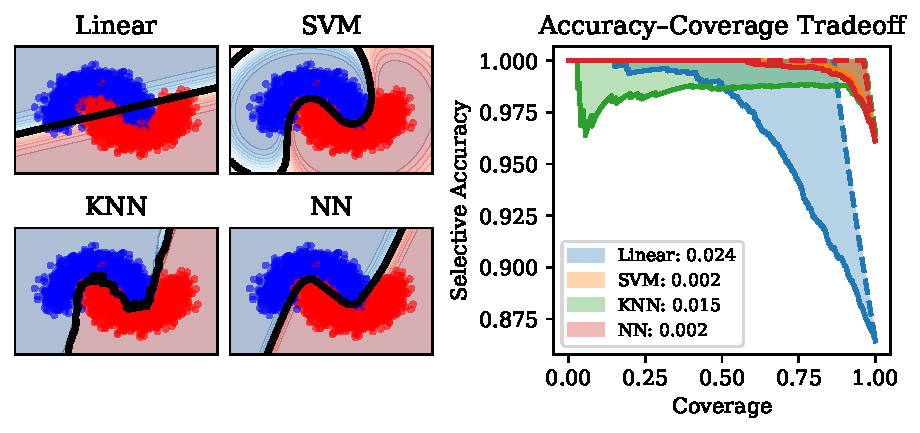
\includegraphics[width=\linewidth]{figs/sc_bounds/2moons_models.pdf}%
    \caption{Approximation error with two moons dataset.}
    \label{fig:left}
  \end{subfigure}%
  \begin{subfigure}[t]{0.24\textwidth}
    \centering
    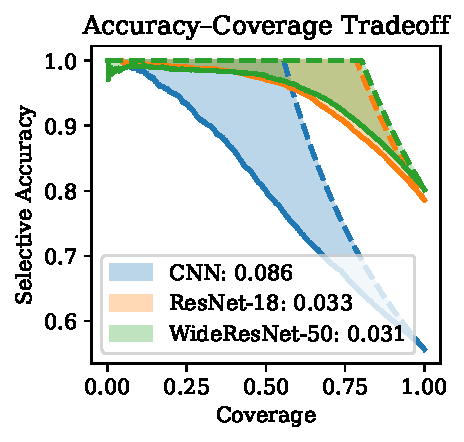
\includegraphics[width=\linewidth]{figs/sc_bounds/cifar100_arch_tradeoffs.pdf} 
    \caption{CIFAR-100}
    \label{fig:right}
  \end{subfigure}
  \begin{subfigure}[t]{0.24\textwidth}
    \centering
    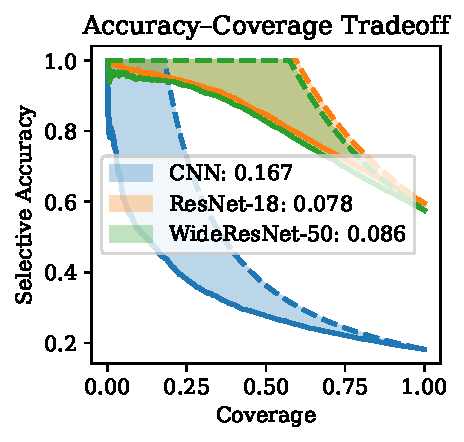
\includegraphics[width=\linewidth]{figs/sc_bounds/stanfordcars_arch_tradeoffs.pdf}
    \caption{StanfordCars}
    \label{fig:right}
  \end{subfigure}
  \caption[Experiments on approximation error.]{\textbf{Experiments on approximation error}. We find that approximation error is a major contributor to the gap. (a) We show the two moons dataset fitted with models of different degrees of expressiveness as well as the corresponding accuracy-coverage tradeoffs. (b) + (c) Accuracy-coverage tradeoffs for various model architectures on CIFAR-100 and StanfordCars, respectively.}
  \label{fig:exp_appr}
\end{figure}

\begin{figure}[t]
  \centering
  % Left: 75% width
  \begin{subfigure}[t]{0.49\textwidth}
  \centering
    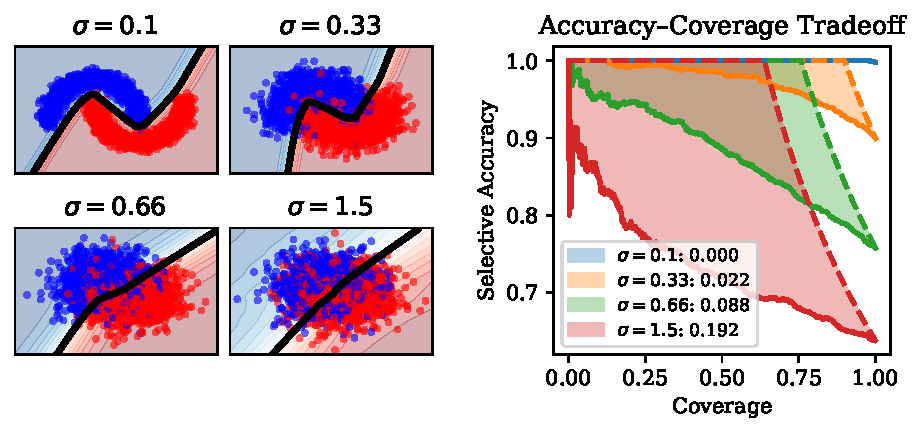
\includegraphics[width=\linewidth]{figs/sc_bounds/2moons_bayes.pdf}%
    \caption{Bayes error with two moons dataset.}
    \label{fig:left}
  \end{subfigure}%
  \begin{subfigure}[t]{0.24\textwidth}
    \centering
    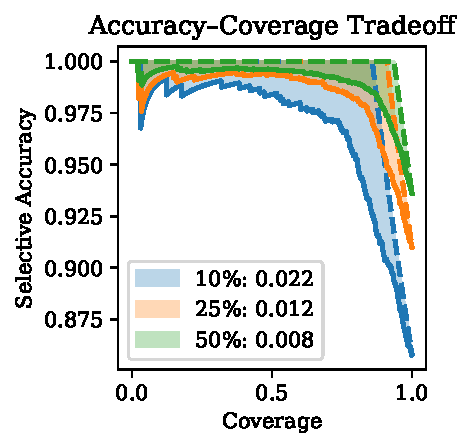
\includegraphics[width=\linewidth]{figs/sc_bounds/cifar10_noisy_tradeoff.pdf}
    \caption{CIFAR-10N}
    \label{fig:right}
  \end{subfigure}
  \begin{subfigure}[t]{0.24\textwidth}
    \centering
    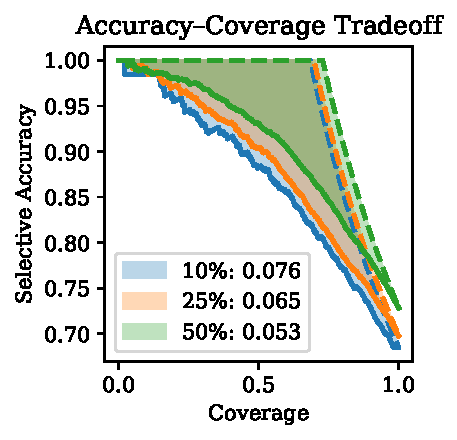
\includegraphics[width=\linewidth]{figs/sc_bounds/cifar100_noisy_tradeoff.pdf}
    \caption{CIFAR-100N}
    \label{fig:right}
  \end{subfigure}
  \caption[Experiments on Bayes error.]{\textbf{Experiments on Bayes error}. We find that irreducible noise significantly contributes to the gap. (a) We show the two moons dataset with varying degrees of noise $\sigma \in \{0.1,0.33,0.66,1.5\}$ as well as the corresponding accuracy-coverage tradeoffs. (b) + (c) Accuracy-coverage tradeoffs for the 10\% (blue), 25\% (orange), and 50\% (green) most noisy images in CIFAR-10N/100N, respectively.}
  \label{fig:exp_bayes}
\end{figure}

\looseness=-1
\emph{Findings.}
In terms of approximation error, Figure~\ref{fig:exp_appr} demonstrates that limited model capacity leads to larger gaps, while more expressive models yield tighter alignment with the perfect-ordering bound. This suggests that approximation error is a key driver of looseness. In terms of Bayes error, Figure~\ref{fig:exp_bayes} shows that increasing label noise consistently shifts the accuracy--coverage curve downward, indicating that Bayes error introduces an irreducible component to the gap. These results validate the canonical bound (Eq.~\ref{eq:emp-gap-ranking})---large Bayes or approximation error can explain substantial looseness.


\begin{table}[t]
\centering
\fontsize{9}{10}\selectfont
\setlength{\tabcolsep}{5pt}
\caption[Experiments on calibration across model classes on CIFAR-100.]{\textbf{Experiments on calibration across model classes on CIFAR-100}. Temperature scaling (\temp) significantly improves ECE over the Maximum Softmax Probability (\msp) baseline but does not help to close the selective classification gap. Self-Adaptive Training (\sat) and Deep Ensembles (\de) improve calibration non-monotonically and also improve selective classification acceptance ordering through re-ranking. A corresponding plot is given in Figure~\ref{fig:cifar100_cal}; more datasets in Tables~\ref{tab:cifar10_cal}, \ref{tab:stanfordcars_cal}.}
\label{tab:cifar100_cal}
\vspace{5pt}
\begin{tabular}{lcccccccccccc}
\toprule
 & \multicolumn{4}{c}{CNN} & \multicolumn{4}{c}{ResNet-18} & \multicolumn{4}{c}{WideResNet-50} \\
\cmidrule(r){2-5} \cmidrule(r){6-9} \cmidrule(r){10-13}
 & \msp & \temp & \sat & \de & \msp & \temp & \sat & \de & \msp & \temp & \sat & \de \\
\midrule
Gap & 0.086 & 0.085 & 0.081 & 0.065 & 0.033 & 0.033 & 0.028 & 0.026 & 0.031 & 0.032 & 0.028 & 0.026 \\
ECE & 0.142 & 0.008 & 0.116 & 0.019 & 0.052 & 0.048 & 0.026 & 0.034 & 0.066 & 0.050 & 0.046 & 0.030 \\
\bottomrule
\end{tabular}
\end{table}

\subsection{Q2: When—and what kind of—calibration helps?}
\label{sec:calibration_ranking_exp}

\emph{Setup.} 
We study the same three model classes as before on CIFAR‑100: a lightweight CNN, a ResNet‑18, and a WideResNet‑50. On each backbone we evaluate the following confidence–scoring variants: (i) maximum softmax probability (\msp)~\citep{hendrycks2016baseline}; (ii) a temperature‑scaled softmax (monotone probability calibration, \temp)~\citep{guo2017calibration}; (iii) self‑adaptive training (\sat)~\citep{huang2020self}, which implicitly calibrates by relabelling uncertain samples during training; and (iv) deep ensembles (\de)~\citep{lakshminarayanan2017simple} of five independently initialised networks (non‑monotone aggregation; improves ranking via variance). For each score we report (i) the weighted Expected Calibration Error (ECE); and (ii) the area enclosed between the empirical accuracy-coverage curve and its perfect-ordering upper bound. i.e., \(\int_0^1 \widehat{\Delta}(c)dc\).

\emph{Findings.}
We summarize our findings in Table~\ref{tab:cifar100_cal}. While temperature scaling (\temp) consistently improves ECE across model classes relative to \msp, it leaves the selective classification gap largely unchanged—highlighting the limitations of monotone calibration. In contrast, \sat slightly improves both ECE and gap by perturbing rankings through relabeling, while deep ensembles (\de) achieve the largest gap reductions by explicitly reordering predictions via averaging. These trends confirm that only methods capable of re-ranking—implicitly (\sat) or explicitly (\de)—can meaningfully improve selective performance. Consistent with this, we find that only \sat and \de models reliably predict their own loss, reinforcing their stronger alignment with correctness. See Appendix~\ref{sec:adv_experiments} for details.


\begin{figure}[t]
  \centering
  % Left: 75% width
  \begin{subfigure}[t]{0.49\textwidth}
  \centering
    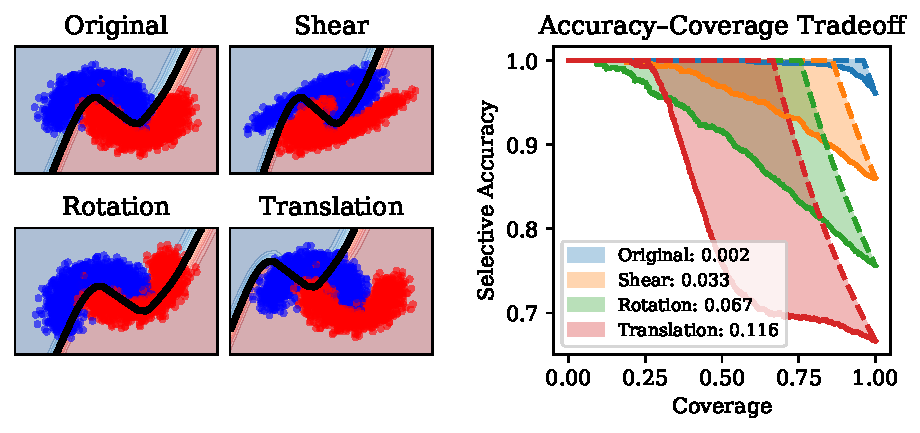
\includegraphics[width=\linewidth]{figs/sc_bounds/2moons_shift.pdf}%
    \caption{Distribution shifts with two moons dataset.}
    \label{fig:left}
  \end{subfigure}%
  \begin{subfigure}[t]{0.24\textwidth}
    \centering
    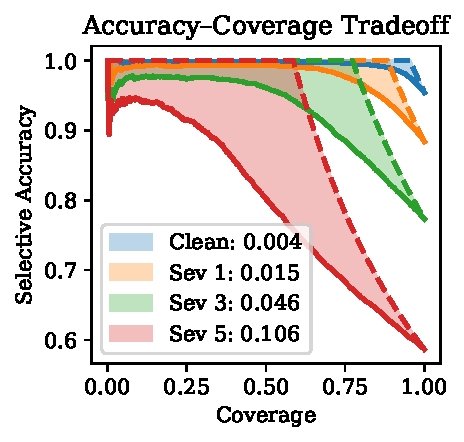
\includegraphics[width=\linewidth]{figs/sc_bounds/cifar10c_tradeoffs.pdf} 
    \caption{CIFAR-10C}
    \label{fig:right}
  \end{subfigure}
  \begin{subfigure}[t]{0.24\textwidth}
    \centering
    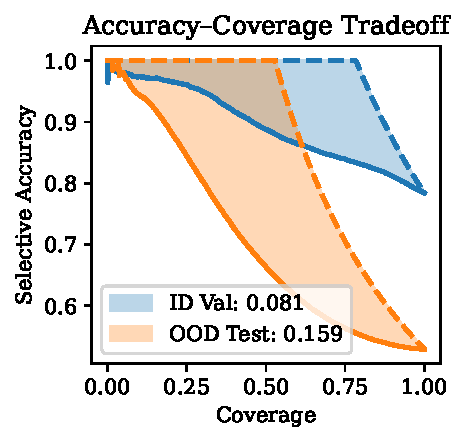
\includegraphics[width=\linewidth]{figs/sc_bounds/camelyon17_tradeoffs.pdf} 
    \caption{Camelyon17-WILDS}
    \label{fig:right}
  \end{subfigure}
  \caption[Experiments on distribution shifts.]{\textbf{Experiments on distribution shifts}. We find that shifts can also significantly contribute to the gap. (a) Two moons under shear, rotation, and translation with corresponding accuracy–coverage curves. (b) CIFAR-10C across three distinct corruption severities. (c) Camelyon17 OOD shift.}
  \label{fig:exp_ds}
\end{figure}

\subsection{Q3: How does the gap evolve under distribution shift?}

\emph{Setup.} As in Q1, we explore this question using both synthetic and real-world distribution shifts. For synthetic experiments, we use the two moons dataset with three types of input shift: shear, rotation, and translation (details in Appendix~\ref{app:twomoons-shifts}). For real data with synthetic corruptions, we use CIFAR-10C~\citep{hendrycks2019robustness}, which applies algorithmic covariate corruptions to the CIFAR-10 test set across five severity levels (1–5). To evaluate under a real distribution shift, we also consider Camelyon17-WILDS~\citep{koh2021wilds}---a cancer detection dataset where test data is collected from a different hospital system than the training data.

\emph{Findings.} Figure~\ref{fig:exp_ds} shows a clear trend: as covariate shifts intensify, the accuracy–coverage curve moves farther below its oracle bound, indicating that abstention no longer isolates easy inputs. Selective classifiers thus become \emph{over-confidently wrong}, echoing evidence that many uncertainty metrics deteriorate under shift or misspecification~\citep{ovadia2019can}. As the gap grows with shift severity, deployments must pair selective prediction with robust ranking or shift-detection safeguards.

\section{Conclusion}
\label{sec:conclusion}

Building a truly performant selective classifier hinges on understanding and closing the gap between practical models and the oracle perfect-ordering bound.  To answer \emph{what it takes}, we introduce a coverage-uniform selective-classification gap and derive the first finite-sample decomposition that pinpoints exactly five limiting factors: three intrinsic sources—Bayes noise, approximation error, and ranking (calibration) error—and two contingent slack terms—sampling variability and implementation or distribution-shift artifacts.  Our experiments show that each component can be individually measured and, importantly, directly improved: stronger model backbones reduce approximation error, non-monotone or feature-aware scoring shrinks ranking error, and shift-robust training with larger validation sets minimizes residual slack.  Together, these insights provide a clear recipe for designing and evaluating high-performance selective classifiers.


\paragraph{Limitations and Future Work.}
While our decomposition cleanly bounds the selective‑classification gap, its error budgets can \emph{interact}—for example, increasing capacity often improves both approximation and ranking—which makes unique attribution challenging. Many \emph{training‑time calibration schemes} (e.g.\ self‑adaptive training, mixup, focal loss) simultaneously affect ranking and full‑coverage accuracy, confounding the separation of budgets. Our experiments focus on \emph{synthetic and vision benchmarks}; extending these insights to language, speech, and large‑scale foundation models would be an important direction. Finally, because our oracle bound and gap are defined for \emph{0–1 loss}, adapting to \emph{asymmetric or class‑dependent cost functions}---often required in high-stakes decision-making---will require generalizing both the bound and its decomposition.  